\section{measurements}
\subsection{Techniques used for the evaluation}
All calculations in this section are done with scripts written in 
the \textit{python} programming language~\cite{python}, relaying in several 
packages:
\begin{itemize}
    \item
        \textit{matplotlib}~\cite{Hunter2007} for plotting,
    \item
        \textit{scipy}~\cite{scipy} for fitting, and 
    \item
        \textit{uncertainties}~\cite{uc} for error propagation.
\end{itemize}
The latter applies gaussian error propagation for correlated and uncorrelated variables. 
We will thus not explicitly write down the formulas for the error propagation 
for each quantity calculated but instead state the numerical result, only. 
We will, however make a quick remark on the use of covariance matrices in 
error propagation: Contrary to measured data, which in our case is usually 
expected to be uncorrelated, all fitted data yields variables that in general correlate. 
The propagation is then done as follows:
Let's assume we have random
variables $x_0,...,x_N$ which are correlated through the $N\times N$ Matrix $cov(x_i,x_j)$.
For a scalar function $f(x_0,...,x_N) \rightarrow \mathbb{R}$, the variance is estimated (linearly) by:
\begin{equation}
Var[f] = \sigma^2 = \sum_{i,j} \frac{\partial f}{\partial x_i} \frac{\partial f}{\partial x_j} cov(x_i,x_j) \,.
\end{equation} 
If instead, $\mathbf{f}$ is a vector field in $m$ dimensions, namely 
$\mathbf{f}(x_0,...,x_N) \rightarrow \mathbb{R}^m$, then the components of $\mathbf{f}$ 
are further correlated. We can write down the relation between the covariance matrices $V$ and $U$ of 
$\mathbf{x}$ and $\mathbf{f}$, respectively, in matrix relations:
\begin{equation}
    U = A V A^T
\end{equation}
where $A$ is the matrix defined by 
\begin{equation}
    A_{ij} = \left[ \frac{\partial f_i}{\partial x_j}\right]_{\mathbf{x} = \mathbf{\mu}}
\end{equation}
with expectation value $E[\mathbf{x}] = \mathbf{\mu}$.~\cite{cowan1998statistical}
In order to facilitate notation, the covariance matrices will in general be notated without 
specifying the units. If not specified explicitly, the units will correspond to those of the
variables: If $x_i, x_j$ have the units $[x_i], [x_j]$, respectively, 
then the entry of the covariance matrix has the unit $[x_i] \cdot [x_j]$. 


\subsection{Calibration and preparation}
As it was already described, we performed the calibration in order to maximize the amplitude of the
signal. The values for the parameters were then  \\
\begin{align*}
     \mathrm{VCA} &= 1355 \qquad \text{(Amplitude of the RLC circuit)}\\
     \mathrm{VCO} &= 1422 \qquad\text{(Frequency of the RLC circuit)}\\ 
     \mathrm{Offset} &= 1680 \qquad\text{(Offset for shifting the signal)}\\
     \mathrm{FB-R} &= 50 k \qquad \text{(Feedback resistor)}
\end{align*}
For the given constraints of the experimental setup see figure~\ref{fig:setup1}.
\begin{figure}[htpb]
    \centering
    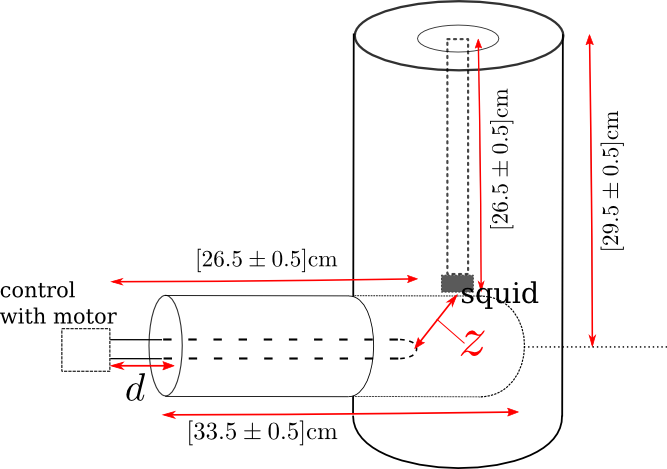
\includegraphics[width=0.8\linewidth]{figures/setup1}
    \caption{Experimental constraints, which we measured before the experimental procedure. The squid
    is connected to the controlling unit, whose output we observe on the oscilloscope. The oscilloscope
    is additionally connected to the computer in order to further analyze the output of the squid.}
    \label{fig:setup1}
\end{figure}
\\\\
We have measured the radius of the coil to 
\begin{equation}
    r = \frac{d}{2} = (2.0 \pm 0.25) \mathrm{mm} \, .
\end{equation}
Using the approximation from equation \eqref{eq:aprox1} we can calculate the
magnetic field $B_z$ and the dipole moment $p$ with 
\begin{align}
B_z     &= \frac{\mu_0\cdot I \cdot r^2}{2z^3} = \frac{\mu_0\cdot U \cdot r^2}{2Rz^3}\\ 
p       &= \pi r^2 U / R 
\end{align}
We approximate the vertical distance of the sensor to the squid to be zero 
for maximal signals. 
The distance between SQUID and sample can then be estimated by
\begin{equation}
z = \left[ 3.0 \pm 0.5 \right]\mathrm{mm}
\end{equation}
The results for the specific resistors used in the experiment are given in the table below. 
\begin{table}[htb]
\caption{
    Calculated magnetic fields of the induction loop with the Biot-Savart law,
    where $R$ denotes to the resistance, $U$ voltage, magnetic field $B_{\mathrm{bs}}$,
    and the dipole moment $p_{\mathrm{bs}}$.
    }
\begin{tabular}{ l| p{2cm}|p{2cm}|p{2cm}|p{2cm}|p{2cm}}
 \rowcolor{tabcolor}& R1 & R2 & R3 & R4 & R5 \\ 
R / $\Omega$ & 51.47  $\pm 0.05$ & 100.8  $\pm 0.1$& 300.8 $\pm 0.3$& 510.6 $\pm 0.3$ & 1000 $\pm 1$\\  
U/V           & 2.63 $\pm 0.01$ & 2.67 $\pm 0.01$& 2.70 $\pm 0.01$& 2.70 $\pm 0.01$& 2.71 $\pm 0.01$\\
$B_{\mathrm{bs}}$ / nT &$4.6 \pm 2.6$&$2.5 \pm 1.4$ &$0.8 \pm 0.5$ &$0.49 \pm 0.28$ &$0.25 \pm 0.14$ \\ 
$p_{\mathrm{bs}}$ / C$\cdot$nm &$620 \pm 150$ &$333 \pm 83$ &$110 \pm 30$ &$66 \pm 17$ &$34 \pm 9$\\
\end{tabular}
\end{table}

\subsection{Measurements with the SQUID}
In order to get a reasonable estimation for the amplitude, we use a least
squares fit with the functional
\begin{equation}
A \cdot \sin (\omega t - \phi ) + c
\end{equation}
with the parameters $A$, $\omega$, $\phi$ and $c$. This parameter space can be
reduced by setting the offset of the data to zero. This is possible by a 
smoothing method: Prior to further analysis, we smooth the data with a
Savitzky-Golay filter%
\footnote{The Savitzky-Golay filter is broadly used
in order to smoothen data without changing the characteristic features of the 
signal. The method is a combination of convolution and polynomial least
squares fitting.} 
in order to subtract the constant $c$. Afterwards, we are left with
\begin{equation}
A \dot \sin (\omega t - \phi ) 
\end{equation}
The other parameters will be given as
a first guess for another least squares fit, now with the real data. This
described method worked very well for us, since the guess of the filtered data
provides the following least squares fit with a good deal of information and
results in a promising fit. The data and fitted sine is shown for 
resistor $R1$ in figure\ref{fig:setup1}. The analogous plots for the 
resistors $R2$ -- $R5$ are shown in the appendix, section~\ref{sec:appendix}.
\begin{figure}[H]
    \centering
    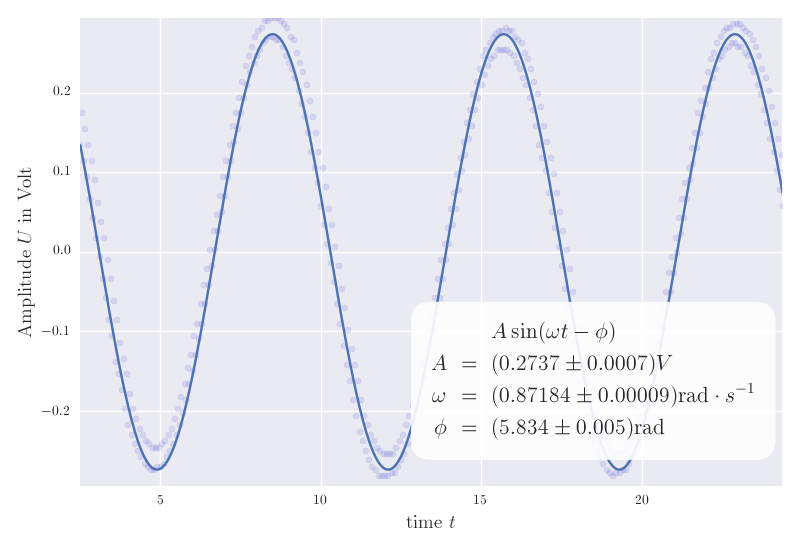
\includegraphics[width=1\linewidth]{analysis/figures/fit4_1}
    \caption{Selected measurement (with resistor R1) in order to visualize the least squares
    fitting. For the other measurements, see the appendix.}
    \label{fig:4_1_plot}
\end{figure}

For calculating the magnetic field, we can use that
the feedback resistor $s_i [V/\phi_0]$ is connected by the effective area $A_{\mathrm{eff}}$
with the magnetic field~\cite{ver}, such that
\begin{equation}
B_z = F \frac{\Delta V}{s_i} \, .
\end{equation}
We used the flux coefficient $F = 9.3$nT$/\phi_0$ (given by the manufacturer) 
which is connected to the effective Area by $F = A_{\mathrm{eff}}^{-1}$. 
The difference in potential is $\Delta V = 2 \cdot A$, 
where $A$ is obtained by fitting the data with the sinus functional. 
The results are given in table~\ref{tab:squid1}.
Attention is be drawn especially to the following factors:
\begin{itemize}
    \item The output of the oscilloscope consists of multiple points shaping a
        whole area of curve (see for instance figure~\ref{fig:4_3_plot}). Is not clear
        whether this is due to a strong fluctuation of the signal or the uncertainty of the
        respective data points, and how we can take this into our considerations 
        for the result and the uncertainty in the end.
    \item From time to time we observed a drift in the signal amplitude. We
        could not retrace the origin of this effect; the result of the fitting 
        resulted hence in an averaging over this drift.
\end{itemize}

Using the already calculated magnetic field, 
the dipole moment is calculated with the same formula as before:
\begin{equation}
    p  = \frac{2 \pi  B_z z^3 }{ \mu_0} \, .
\end{equation}
Since this expression is strongly influenced by the value of $z$, we expect a large error 
stemming from the large error on $z$. 
For the calculated values, refer to table~\ref{tab:squid1}. 
\begin{table}[htb]
\caption{
    Calculated magnetic fields with by the SQUID, where ``sq'' denotes to SQUID method. 
    Here we show the
    amplitude $A$, magnetic field $B_{\mathrm{sq}}$ and the dipole 
    moment $p_{\mathrm{sq}}$. We again emphasize the
    big error on $p_{\mathrm{sq}}$ coming from the rather uncertain 
    value of $z$ and the very tiny error on the magnetic field. 
    For the respective figures please see the appendix, section~\ref{sec:appendix}.}
\begin{tabular}{ l| p{2.3cm}|p{2.3cm}|p{2.3cm}|p{2.3cm}|p{2.3cm}}
    \rowcolor{tabcolor}
        & R1 & R2 & R3 & R4 & R5 \\ 
    R / $\Omega$ & 50  $\pm 1$ & 100  $\pm 1$   &
        300  $\pm 1$& 500 $\pm 1$ & 1000 $\pm 1$    \\  
    A / mV &$273.7 \pm 0.7$&$142.1 \pm 0.6$&
        $48.2 \pm 0.5$&$27.9 \pm 0.5$&$15.4 \pm 0.7$    \\
    $B_{\mathrm{sq}}$ / nT &$5.09 \pm 0.12$&$2.64 \pm 0.06$&    
        $0.896 \pm 0.022$&$0.519 \pm 0.015$&$0.286 \pm 0.014$   \\  
    $p_{\mathrm{sq}}$/ C$\cdot$nm &$690 \pm 140$ & $360 \pm 70$ &
        $121 \pm 24$ & $70 \pm 14$ & $39 \pm 8$     \\
\end{tabular}
\label{tab:squid1}
\end{table}
In order to relate these results to the former ones obtained with the Biot-Savart law, we compare 
both of them in table~\ref{tab:comparison}. 
Evidently the SQUID method is able to resolve the magnetic field with a 
much greater precision. This is above all due to the large
error measuring the distance sample -- Squid $z$. 
We thus conclude that the SQUID method is far better at measuring magnetic fields 
when compared to the method of applying Biot-Savart's law. 
In our case, the precision exploiting superconductivity 
and the Josephson junction leads to a precision of three orders of magnitude 
better than the classical electro dynamical approach. 
\begin{table}[htb]
\caption{Comparison of the two methods. ``bs'' refers to Biot-Savart law, 
    ``sq'' to the SQUID method. Note the great differences in precision between 
    the two methods for the magnetic field.}
\begin{tabular}{ l| p{2.3cm}|p{2.3cm}|p{2.3cm}|p{2.3cm}|p{2.3cm}}
 \rowcolor{tabcolor}& R1 & R2 & R3 & R4 & R5 \\ 
$B_{\mathrm{bs}}$ / nT &$4.6 \pm 2.6$&$2.5 \pm 1.4$ &$0.8 \pm 0.5$ &$0.49 \pm 0.28$ &$0.25 \pm 0.14$ \\ 
$p_{\mathrm{bs}}$ / C$\cdot$nm &$620 \pm 150$ &$333 \pm 83$ &$110 \pm 30$ &$66 \pm 17$ &$34 \pm 9$\\
$B_{\mathrm{sq}}$ / nT &$5.09 \pm 0.12$&$2.64 \pm 0.06$&$0.896 \pm 0.022$&$0.519 \pm 0.015$&$0.286 \pm 0.014$\\  
$p_{\mathrm{sq}}$/ C$\cdot$nm &$690 \pm 140$ & $360 \pm 70$ &$121 \pm 24$ & $70 \pm 14$ & $39 \pm 8$ \\
\end{tabular}
\label{tab:comparison}
\end{table}
\FloatBarrier
\subsection{Measuring various materials}
After measuring the rather stable signal of the induction loop, we tried to measure
the magnetic field and dipole moments of various other materials. 
The measured signals were to a great extent worse than the signals of the induction loop,
as can be observed in the figures in the appendix, section~\ref{sec:appendix}. 
Nevertheless, we were able to capture the characteristic features of the curves. 
We calculated the magnetic fields (see table~\ref{tab:materials}), with the following limitations: 
\begin{itemize}
    \item We were not sure how to include the various shapes into the propagation of the error, since
        we expected a clear sinus signal. In those cases, when it was not possible at all to fit a sinus
        to the signal, we took the amplitude of a filtered curve for the calculation of the magnetic field, with
        an estimated error of 10\%. %
        \footnote{in particular, in measurement 5.1 (Gold), 5.2 (Iron) and 5.3 (Gold).
        Measurements 5.4 (Stick) and 5.5 (Magnetic splint) were fitted with a sinus functional.}
    \item We have no further information of how
        the shape of the signal should be included. These results should not be considered to be very precise.
        We are convinced that this method yields not more than an estimation of the order
        of magnitude of the magnetic field.
    \item In the former section we calculated the distance $z$ between the induction loop and the 
        SQUID. Clearly, the assumptions made before are not valid any more, such that the approximation 
        becomes much more uncertain in the case of samples with various sizes. It is
        unclear how the size of the object influences can be considered in both the estimation of the 
        dipole moments and the error propagation. De decided to apply the following procedure:
        We assume the distance $z$ still to be the same as before, only in order to be able to 
        compares this values with the formers but with the knowledge that this distance is actually not 
        possible. We have to emphasize that the calculation of the dipole moments is not meaningful
        in this case and the results should not referred to as precise results.
\end{itemize}

\begin{table}[htb]
\caption{Measuring the magnetic field of different materials. 
    Note the change in units for the dipole moment.}
\begin{tabular}{ l| p{2.3cm}|p{2.3cm}|p{2.3cm}|p{2.3cm}|p{2.3cm}}
 \rowcolor{tabcolor}& Gold & Iron & Gold  & Stick & Magnet splint \\ 
Amplitude / V &$0.046 \pm 0.005$&$0.054 \pm 0.005$&$0.051 \pm 0.005$&$3.72 \pm 0.05$&$6.94 \pm 0.04$\\
$B_{\mathrm{sq}}$ / nT  &$0.86 \pm 0.09$ &$1.00 \pm 0.10$ &$0.95 \pm 0.10$ &$69.2 \pm 1.8$ &$129.2 \pm 3.0$ \\ 
$p_{\mathrm{sq}}$ / C$\cdot\mu$m  &$0.116 \pm 0.026$&$0.136 \pm 0.030$&$0.128 \pm 0.029$&$9.3 \pm 1.9$&$17 \pm 4$\\
\end{tabular}
\label{tab:materials}
\end{table}
\FloatBarrier
\subsection{Polar plots}
In order to visualize the spatial dependence of the magnetic field on both the 
induction loop and the other materials, we use a specific way of plotting 
our data called \textit{polar plot}. Since we are measuring a more or less
continuous signal in time and since we can estimate the rotational state
of the object, it is possible to relate the amplitude to the respective magnetic
field. Hence, we use the following transformation:
\begin{align}
    B_x = |A - \bar{A}| \cos(\omega t) \\
    B_y = |A - \bar{A}| \sin(\omega t) 
\end{align}
where $\bar{A}$ denotes to the mean with respect to the timespan we are looking at.
Since our signal was not that stable, we plotted multiple periods ($\Delta t = 6T$) in 
order to get an idea about the fluctuations. Otherwise we would have had only
an incomplete picture about our measurements. Our result is the following:
For intense magnetic fields we can differentiate the shape of the magnetic field
in a good way; for the others noise and the systematic errors disturb our
signal such that it is not possible to relate the polar plot to the physical reality. 
\begin{figure}[H]
    \centering
    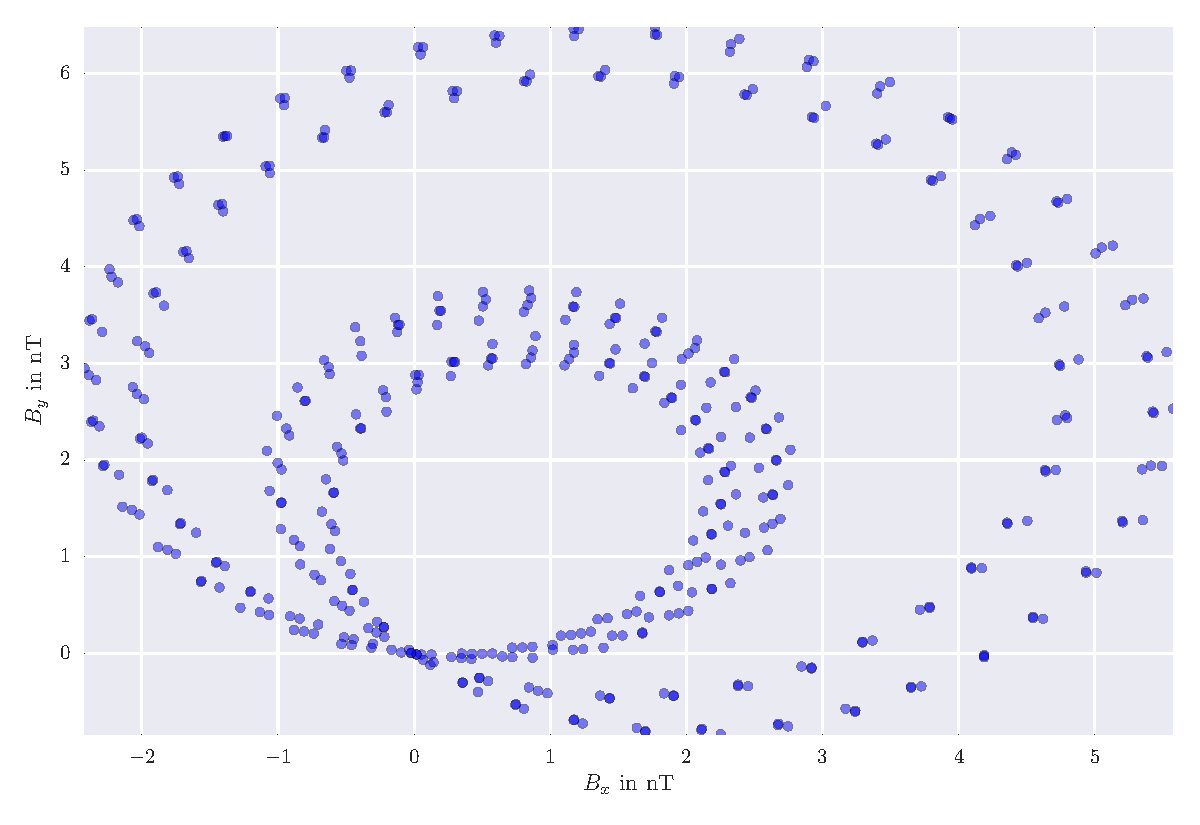
\includegraphics[width=1\linewidth]{analysis/figures/polar4_1}
    \caption{Selected measurement (R1) in order to visualize the polar plot.
    For the other measurements please see the appendix.}
    \label{fig:4_1_polar}
\end{figure}

